%!TEX root = ../thesis.tex

\section{地図を用いたルールベース制御器によるナビゲーション}
先行研究と提案手法において, 教師信号としている地図を用いたルールベース制御器によるナビゲーションについて説明する. このナビゲーションには, ROSのパッケージであるnavigation\cite{navigation}を使用している. 移動ロボットは, \figref{Fig:navigation}のようにLiDARのスキャンデータやオドメトリを入力として自己位置推定と経路計画を行い, これらに基づいて自律走行をする. また, 自己位置推定には, amcl(Adaptive Monte Carlo Localization), 経路計画とモータ指令にはmove\_base\cite{navigation}を使用している. 

\begin{figure}[h]
     \centering
     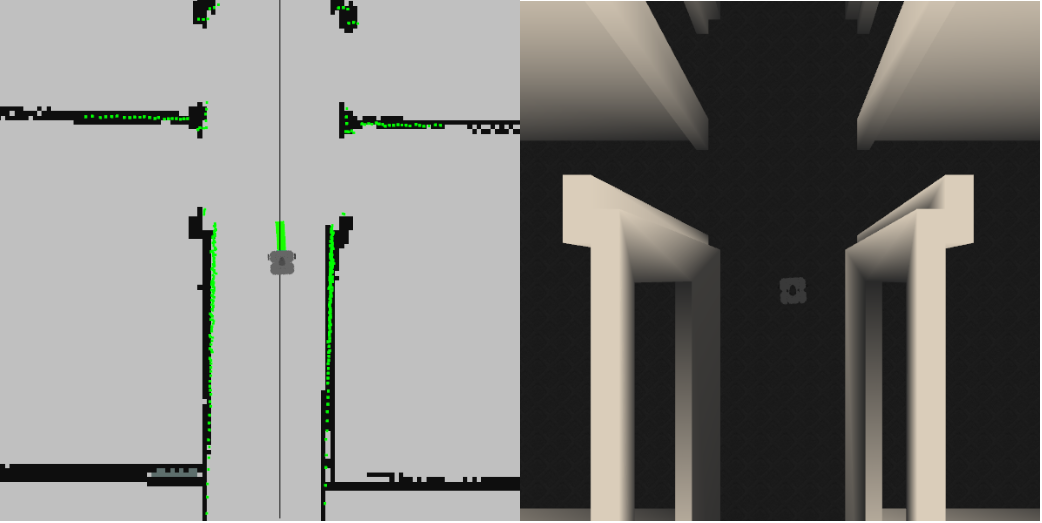
\includegraphics[keepaspectratio, scale=0.3]
     {images/navigation.png}
     \caption{Map based navigation using navigation package}
     \label{Fig:navigation}
     \end{figure}

\section{ディープラーニング}
ディープラーニングとは, 人間の神経細胞を模したネットワーク構造のことである. 主に, 入力層と出力層, その間に中間層(隠れ層)という構成である. 中間層を多層化することで, 複雑な入力情報を処理し, パターンを認識することや, ルールを読み解くことができる. 近年では, 画像や物体認識, 自然言語処理などで活用されている. \figref{Fig:dl}に構造の一例を示す. 

\vspace{30mm}

\begin{figure}[h]
     \centering
     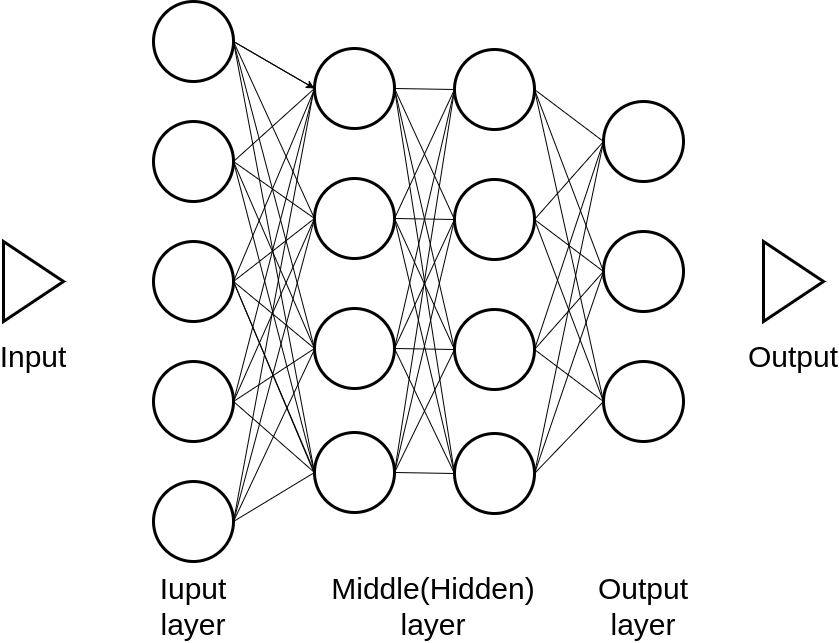
\includegraphics[keepaspectratio, scale=0.3]
     {images/dl.png}
     \caption{Structure of Deep Learning}
     \label{Fig:dl}
     \end{figure}

\newpage
\section{end-to-end学習}
end-to-end学習とは, 入力から出力までの流れを一括に学習することができる手法である. 例として, 画像中からの文字認識を行う処理を挙げる. 一般的な処理では, \figref{Fig:example}のように画像から文字検出を行い, その後に文字分割, 最終的に文字認識をする. しかし, end-to-end学習では, \figref{Fig:end-to-end}に示すような入力から出力までの流れを一括して学習することができる. 

\vspace{35mm}

\begin{figure}[h]
     \centering
     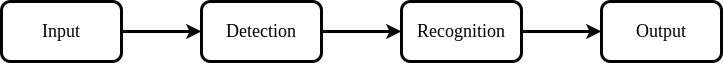
\includegraphics[keepaspectratio, scale=0.5]
     {images/example.png}
     \caption{Structure of general Learning}
     \label{Fig:example}
     \end{figure}

\begin{figure}[h]
     \centering
     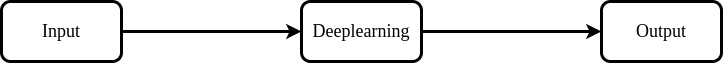
\includegraphics[keepaspectratio, scale=0.5]
     {images/end-to-end.png}
     \caption{Structure of end-to-end Learning}
     \label{Fig:end-to-end}
     \end{figure}

\newpage
\section{データセット}
データセットとは, 学習に使用する学習(訓練)データの集合のことである. 例として, \figref{Fig:mnist}に示すような0から9の手書きで書かれた数字の画像セットであるMNISTが挙げられる. 機械学習や画像認識において多く利用されており, 訓練画像6000枚とテスト画像1000枚で構成されている. 

\vspace{5mm}

\begin{figure}[h]
     \centering
     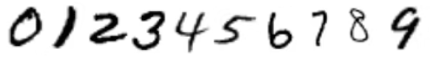
\includegraphics[keepaspectratio, scale=0.5]
     {images/mnist.png}
     \caption{MNIST dataset from \cite{mnist}}
     \label{Fig:mnist}
     \end{figure}

\section{模倣学習におけるオフライン}
模倣学習におけるオフラインとは, あらかじめ用意したデータセットを使用して学習を行うことである. これに対して, 先行研究用で用いた模倣学習におけるオンラインとは, タスクを行いながらデータ収集をし, そのデータを使用して学習することを指す. 

\section{ミニバッチ学習}
ミニバッチ学習とは, 訓練データをいくつかのグループ(バッチ)に分けて順番に学習を行うことである. 特徴としては, 勾配更新の頻度が高く, 計算量が少なくて済むといったことが挙げられる. これらの特徴を踏まえて, 先行研究ではオンラインで学習を行うことから, ミニバッチ学習を使用している.
\section{バッチ学習}
バッチ学習とは, 訓練データを一括で処理する学習方法である. 特徴として, 一度に大量のデータを扱うことができるため学習の進行が安定しやすく, 訓練データに異常データが混じっていても受ける影響が小さくて済むなどが挙げられる. 